\documentclass[11pt,a4paper]{article}
\usepackage[margin=2.3cm]{geometry}
\usepackage{mathptmx}            % Times text and math
\DeclareSymbolFont{symbols}{OMS}{cmsy}{m}{n}  % mathptmx's OMS virtual font takes \mathcal from rsfs, which minimal TeX installs lack;
                                              % pdftex then drops every \F and \LL glyph. CM symbols carry the same calligraphic letters.
\usepackage[T1]{fontenc}
\usepackage[utf8]{inputenc}
\usepackage{amsmath,amssymb,bm}
\usepackage{booktabs,graphicx,caption,subcaption}
\usepackage[round,sort]{natbib}
\usepackage[hidelinks]{hyperref}
\usepackage{url}
\usepackage{microtype}
\captionsetup{font=small,labelfont=bf,skip=4pt}
\setlength{\parskip}{3pt}
\setlength{\abovedisplayskip}{4pt}\setlength{\belowdisplayskip}{4pt}
\setlength{\abovedisplayshortskip}{2pt}\setlength{\belowdisplayshortskip}{2pt}
\setlength{\textfloatsep}{8pt}\setlength{\intextsep}{8pt}
\newcommand{\DataStart}{2014-02-01}
\newcommand{\DataEnd}{2026-05-23}
\newcommand{\DataT}{4495}
\newcommand{\OOSStart}{2018-01-31}
\newcommand{\OOSEnd}{2026-05-23}
\newcommand{\NWindows}{34}
\newcommand{\TrainLen}{1460}
\newcommand{\TestLen}{91}
\newcommand{\NOOS}{3035}
\newcommand{\TargetVol}{20}
\newcommand{\WMax}{1}
\newcommand{\CostBps}{10}
\newcommand{\LRlogrv}{198.3}
\newcommand{\LRexflow}{5.7}
\newcommand{\LRexflowP}{0.058}
\newcommand{\LRboth}{205.6}
\newcommand{\LRkthree}{163.6}
\newcommand{\SigCalm}{33}
\newcommand{\SigTurb}{105}
\newcommand{\SigCalmT}{30}
\newcommand{\SigTurbT}{105}
\newcommand{\BetaOneRV}{-0.914}
\newcommand{\BetaOneRVse}{0.120}
\newcommand{\BetaTwoRV}{1.251}
\newcommand{\BetaTwoRVse}{0.224}
\newcommand{\PstayCalm}{0.899}
\newcommand{\PstayTurb}{0.812}
\newcommand{\DurCalm}{9.9}
\newcommand{\DurTurb}{5.3}
\newcommand{\BICtwo}{-18678}
\newcommand{\BICthree}{-18896}
\newcommand{\BICtvtp}{-18859}
\newcommand{\WFfracLR}{100}
\newcommand{\WFfracBIC}{100}
\newcommand{\WFmedLR}{63.8}
\newcommand{\WFfracLRex}{0}
\newcommand{\SlopeOneMin}{-1.33}
\newcommand{\SlopeOneMax}{-0.43}
\newcommand{\SlopeTwoMin}{0.37}
\newcommand{\SlopeTwoMax}{1.80}
\newcommand{\DMqlike}{-2.27}
\newcommand{\DMqlikeP}{0.023}
\newcommand{\DMmse}{-2.55}
\newcommand{\DMmseP}{0.011}
\newcommand{\DMls}{-4.62}
\newcommand{\DMlsP}{$<$0.001}
\newcommand{\DMewmaQ}{-1.22}
\newcommand{\DMewmaQP}{0.223}
\newcommand{\DMrvQ}{-4.37}
\newcommand{\DMrvQP}{$<$0.001}
\newcommand{\SRbh}{0.71}
\newcommand{\SRvt}{0.59}
\newcommand{\SRhmm}{0.39}
\newcommand{\SRtvtp}{0.61}
\newcommand{\TOhmm}{16.5}
\newcommand{\TOtvtp}{9.2}
\newcommand{\MDDbh}{-77}
\newcommand{\MDDtvtp}{-25}
\newcommand{\VolTvtp}{11}
\newcommand{\SRhmmK}{0.52}
\newcommand{\SRtvtpK}{0.76}
\newcommand{\MDDtvtpK}{-55}
\newcommand{\VolTvtpK}{37}
\newcommand{\WealthBH}{7.7}
\newcommand{\WealthTvtpK}{5.9}
\newcommand{\BootDiff}{0.22}
\newcommand{\BootLo}{-0.05}
\newcommand{\BootHi}{0.49}
\newcommand{\BootP}{0.107}
\newcommand{\PSR}{0.96}
\newcommand{\DSR}{0.84}
\newcommand{\NTrials}{54}
\newcommand{\SRzero}{0.26}
\newcommand{\BootDiffK}{0.25}
\newcommand{\BootLoK}{0.00}
\newcommand{\BootHiK}{0.47}
\newcommand{\BootPK}{0.050}
\newcommand{\PSRK}{0.99}
\newcommand{\DSRK}{0.92}
\newcommand{\GapZero}{0.16}
\newcommand{\GapFifty}{0.46}
\newcommand{\SynN}{200}
\newcommand{\SynT}{2000}
\newcommand{\SynCovMin}{0.925}
\newcommand{\SynCovMax}{0.965}
\newcommand{\SynSizeTen}{0.100}
\newcommand{\SynSizeFive}{0.050}
\newcommand{\SynSizeOne}{0.010}
\newcommand{\SynKS}{0.07}
\newcommand{\SynPower}{1.00}
\newcommand{\SynAccS}{93}
\newcommand{\SynAccF}{90}
\newcommand{\SynIntN}{100}
\newcommand{\SynIntCovMin}{0.89}
\newcommand{\SynIntCovMax}{0.95}
\newcommand{\LRlogrvHalf}{99}
\newcommand{\CrossVol}{72}
\newcommand{\LowVol}{16}
\newcommand{\LowPcalm}{0.94}
\newcommand{\LowDurCalm}{16}
\newcommand{\LowDurTurb}{1.0}
\newcommand{\HighVol}{155}
\newcommand{\HighPturb}{0.88}
\newcommand{\HighDurTurb}{8}
\newcommand{\HighDurCalm}{1.4}
\newcommand{\FTXfirst}{2022-11-04}
\newcommand{\FTXpre}{0.08}
\newcommand{\COVIDfirst}{2020-03-02}
\newcommand{\COVIDpre}{0.74}
\newcommand{\KthreeWFfracLR}{100}
\newcommand{\KthreeWFfracBIC}{85}
\newcommand{\KthreeDMqlike}{-1.43}
\newcommand{\KthreeDMqlikeP}{0.152}
\newcommand{\KthreeDMls}{-4.05}
\newcommand{\KthreeDMlsP}{$<$0.001}
\newcommand{\KthreeSRhmm}{0.54}
\newcommand{\KthreeSRtvtp}{0.50}
\newcommand{\KthreeSRhmmK}{0.68}
\newcommand{\KthreeSRtvtpK}{0.63}
\newcommand{\KthreeBootLo}{-0.29}
\newcommand{\KthreeBootHi}{0.23}
\newcommand{\KthreeBootP}{0.811}
\newcommand{\KthreeBootLoK}{-0.25}
\newcommand{\KthreeBootHiK}{0.17}
\newcommand{\KthreeBootPK}{0.657}
\newcommand{\KthreeDMmse}{-2.16}
\newcommand{\KthreeDMmseP}{0.031}
\newcommand{\TLLhmm}{9537.9}
\newcommand{\TLLtvtp}{9553.2}
\newcommand{\TBIChmm}{-19009}
\newcommand{\TBICtvtp}{-19022}
\newcommand{\TLR}{30.6}
\newcommand{\TLRex}{7.3}
\newcommand{\TLRexP}{0.026}
\newcommand{\TNuCalm}{3.1}
\newcommand{\TNuTurb}{5.2}
\newcommand{\TNuCalmH}{2.7}
\newcommand{\TNuTurbH}{4.1}
\newcommand{\TSigCalm}{38}
\newcommand{\TSigTurb}{92}
\newcommand{\TBetaOne}{-1.05}
\newcommand{\TBetaOneSE}{0.25}
\newcommand{\TBetaTwo}{1.52}
\newcommand{\TBetaTwoSE}{0.31}
\newcommand{\TWFfracLR}{62}
\newcommand{\TWFfracBIC}{12}
\newcommand{\TWFmedLR}{6.9}
\newcommand{\TSlopeOneMin}{-1.45}
\newcommand{\TSlopeOneMax}{1.93}
\newcommand{\TSlopeOneMed}{-0.42}
\newcommand{\TSlopeTwoMin}{-1.72}
\newcommand{\TSlopeTwoMax}{2.04}
\newcommand{\TSlopeTwoMed}{0.91}
\newcommand{\TLShmm}{2.1395}
\newcommand{\TLStvtp}{2.1381}
\newcommand{\TDMls}{0.53}
\newcommand{\TDMlsP}{0.598}
\newcommand{\TDMqlike}{-0.81}
\newcommand{\TDMqlikeP}{0.420}
\newcommand{\TDMmse}{2.11}
\newcommand{\TDMmseP}{0.035}
\newcommand{\TSRhmm}{0.53}
\newcommand{\TSRtvtp}{0.43}
\newcommand{\TSRhmmK}{0.52}
\newcommand{\TSRtvtpK}{0.56}
\newcommand{\TBootLo}{-0.47}
\newcommand{\TBootHi}{0.26}
\newcommand{\TBootP}{0.599}
\newcommand{\TBootLoK}{-0.22}
\newcommand{\TBootHiK}{0.27}
\newcommand{\TBootPK}{0.794}
\newcommand{\GLStvtp}{2.1196}
\newcommand{\GLShmm}{2.0996}
\newcommand{\StudentTText}{With Student-$t$ emissions (regime-specific degrees of freedom $\nu_j$, estimated by an ECM step inside EM and polished by quasi-Newton; the regime variance is $\sigma_j^2\nu_j/(\nu_j-2)$ and enters (\ref{eq:fc}) in place of $\sigma_j^2$) the picture changes more sharply. On the full sample the constant $t$-HMM reaches a log-likelihood of \TLLhmm\ (BIC \TBIChmm), better than any Gaussian model including the three-regime ones, with $\hat\nu=(\TNuCalmH, \TNuTurbH)$: the calm regime is very heavy-tailed. Adding realised volatility to the transitions is still significant, LR $=\TLR$ on two degrees of freedom, with slopes of the hypothesised sign and larger magnitude ($\beta_{1,\mathrm{RV}}=\TBetaOne$ (\TBetaOneSE), $\beta_{2,\mathrm{RV}}=\TBetaTwo$ (\TBetaTwoSE)), and the exchange-flow effect becomes marginally significant (LR $=\TLRex$, $p=\TLRexP$). Out of sample, however, the effect does not survive. In rolling four-year windows the LR test rejects in only \TWFfracLR\% of windows (median LR \TWFmedLR), BIC prefers the TVTP model in \TWFfracBIC\%, and the slopes are unstable ($\beta_{1,\mathrm{RV}}$ ranges from \TSlopeOneMin\ to \TSlopeOneMax\ across windows, median \TSlopeOneMed). The $t$-HMM's own predictive log score (\TLShmm) already exceeds that of the Gaussian TVTP model (\GLStvtp), and the $t$-TVTP model adds nothing to it (\TLStvtp, DM $t=\TDMls$, $p=\TDMlsP$); its variance forecasts are no better under QLIKE ($t=\TDMqlike$, $p=\TDMqlikeP$) and worse under MSE ($t=\TDMmse$, $p=\TDMmseP$). Sharpe ratios are \TSRtvtp\ against \TSRhmm\ under the proportional rule ([\TBootLo, \TBootHi], $p=\TBootP$) and \TSRtvtpK\ against \TSRhmmK\ under Kelly ([\TBootLoK, \TBootHiK], $p=\TBootPK$). Full tables are in the repository (\texttt{results/btc\_t/}).}
\newcommand{\XDMtls}{-1.88}
\newcommand{\XDMtlsP}{0.061}
\newcommand{\XDMkls}{0.15}
\newcommand{\XDMklsP}{0.88}
\newcommand{\NTrialsAll}{162}
\newcommand{\DSRpooled}{0.85}
\newcommand{\DSRKpooled}{0.93}
\newcommand{\KthreeText}{Repeating the walk-forward exercise with $K=3$ (calm, intermediate and turbulent regimes, six transition slopes, EM without the quasi-Newton polish) gives the following. The realised-volatility TVTP model rejects the constant three-regime HMM in \KthreeWFfracLR\% of windows and has the lower BIC in \KthreeWFfracBIC\%. Against the three-regime baseline the Diebold--Mariano statistics are $t=\KthreeDMqlike$ for QLIKE ($p=\KthreeDMqlikeP$), $t=\KthreeDMmse$ for MSE ($p=\KthreeDMmseP$) and $t=\KthreeDMls$ for the log score ($p\KthreeDMlsP$). Under the proportional rule with $a=(1,\tfrac12,0)$ in (\ref{eq:rule}) the Sharpe ratios are \KthreeSRtvtp\ (TVTP) and \KthreeSRhmm\ (constant HMM), bootstrap interval for the difference [\KthreeBootLo, \KthreeBootHi] ($p=\KthreeBootP$); under the Kelly rule \KthreeSRtvtpK\ against \KthreeSRhmmK\ ([\KthreeBootLoK, \KthreeBootHiK], $p=\KthreeBootPK$). Full tables are in the repository (\texttt{results/btc\_k3/}).}


\newcommand{\F}{\mathcal{F}}
\newcommand{\bxi}{\bm{\xi}}
\newcommand{\bP}{\mathbf{P}}
\newcommand{\beeta}{\bm{\eta}}
\newcommand{\bbeta}{\bm{\beta}}
\newcommand{\LL}{\mathcal{L}}
\DeclareMathOperator{\Lam}{\Lambda}

\title{\vspace{-1.2cm}Regime detection in Bitcoin volatility with a time-varying-transition-probability hidden Markov model and a regime-conditioned allocation rule}
\author{Alaa Breim\\[2pt]
\small Final Degree Project, Applied Artificial Intelligence and its Mathematical Foundations\\
\small University of the Basque Country - EHU
}
\date{September 2026}

\begin{document}
\maketitle
\vspace{-0.8cm}
\begin{abstract}
\noindent
Bitcoin returns alternate between calm and turbulent volatility regimes. The standard tool for identifying them, a hidden Markov model (HMM) estimated with the Hamilton filter, assumes constant regime-transition probabilities. This project extends the HMM with time-varying transition probabilities (TVTP) driven by an observable covariate, derives the modified filter, smoother and expectation-maximisation step, and asks whether the extension improves regime forecasts and downstream trading in a statistically significant sense rather than only in fit. Two covariates are considered: lagged realised volatility and on-chain exchange net-flow. The estimator is validated by Monte Carlo (parameter recovery, confidence-interval coverage, and the exact size of the nested likelihood-ratio test). On daily data from \DataStart\ to \DataEnd, realised volatility strongly modulates regime persistence: the calm regime becomes less persistent and the turbulent regime more persistent as volatility rises, and the TVTP model rejects the constant HMM in every one of \NWindows\ walk-forward windows. Out of sample, one-day-ahead variance and density forecasts improve significantly by Diebold--Mariano tests (QLIKE $t=\DMqlike$, log score $t=\DMls$). With two regimes, a regime-conditioned, volatility-scaled allocation rule fed by the TVTP model raises the Sharpe ratio from \SRhmm\ to \SRtvtp\ relative to the constant-HMM rule with roughly half the turnover; stationary-bootstrap intervals for the difference are [\BootLo, \BootHi] ($p=\BootP$) and, under a capped-Kelly rule, [\BootLoK, \BootHiK] ($p=\BootPK$), with deflated Sharpe ratios of \DSR\ and \DSRK\ after accounting for \NTrials\ configurations tried. These gains are specific to the two-regime Gaussian baseline. With three regimes the density-forecast gain survives but the trading gain does not; with Student-$t$ emissions the effect remains significant in the full sample (LR $=\TLR$) but the $t$-HMM alone forecasts at least as well out of sample as any Gaussian model and time variation adds nothing further. Realised volatility in the transition probabilities is therefore a real feature of Bitcoin regime dynamics, but much of its forecasting value is a substitute for, not a complement to, a richer emission distribution. Exchange net-flow carries no out-of-sample information. Code, data pipeline and all results are in the companion repository.
\end{abstract}

\section{Introduction}
Volatility clustering and heavy tails are the defining stylised facts of asset returns \citep{cont2001}, and Bitcoin exhibits both in extreme form: annualised volatility moves between roughly 30\% and above 100\% within weeks, and episodes such as the March 2020 liquidation, the May 2022 Terra collapse and the November 2022 FTX failure arrive as abrupt shifts rather than gradual drifts. Regime-switching models describe such behaviour by a latent Markov chain that selects among a small number of return distributions \citep{hamilton1989}. In their standard form the chain is time-homogeneous: the probability of leaving the calm regime tomorrow is the same whether the market has been placid or already unsettled. That assumption is convenient for estimation but implausible for a market whose stress is partly observable in advance.

This project relaxes it. Following \citet{filardo1994} and \citet{dlw1994}, the transition matrix is made a logistic function of a covariate observed one day earlier, which keeps every quantity used for forecasting measurable with respect to the previous close. The research question is whether this extension improves (i) regime and volatility forecasting quality and (ii) the performance of a simple regime-conditioned, volatility-scaled allocation rule, relative to the constant-transition HMM baseline, by margins that survive formal significance testing rather than only in-sample fit.

The contributions are as follows. First, a complete derivation of the Hamilton filter, Kim smoother and Baum--Welch algorithm for the Gaussian HMM, and of the one-line modification and the generalised EM step that the TVTP extension requires, in a single notation matched line by line by the implementation. Second, a Monte Carlo validation of the estimator, including the empirical size of the nested likelihood-ratio test, which is regular here unlike the test for the number of regimes. Third, an out-of-sample evaluation on Bitcoin under strict walk-forward validation, combining Diebold--Mariano tests on variance and density forecasts with bootstrap inference and deflated Sharpe ratios on a backtested allocation rule. The combination of a modern covariate, a fully causal trading rule and formal significance testing is what distinguishes the project from prior TVTP work on Bitcoin, which stops at in-sample fit and one-step forecast accuracy.

Section~\ref{sec:related} places the project in the literature, Section~\ref{sec:method} derives the models and estimators, Section~\ref{sec:design} describes data and experimental design, Section~\ref{sec:results} reports results, and Sections~\ref{sec:discussion} and \ref{sec:conclusion} discuss and conclude.

\section{Related work}\label{sec:related}
\paragraph{Conditional heteroskedasticity.} The ARCH model of \citet{engle1982} and its GARCH generalisation \citep{bollerslev1986} describe volatility clustering through a recursion on past squared shocks; the EGARCH \citep{nelson1991} and GJR \citep{gjr1993} variants add the leverage asymmetry. For Bitcoin, \citet{katsiampa2017} compares GARCH-family fits and finds that a component model with separate short- and long-run variance terms fits best, a first sign that a single decay rate does not describe the series.

\paragraph{Regime switching.} \citet{hamilton1989} introduced the Markov-switching model and the filter that computes regime probabilities and the likelihood recursively; \citet{kim1994} added the smoother used inside EM. In the signal-processing literature the same objects appear as the forward--backward and Baum--Welch algorithms \citep{baum1970,rabiner1989,viterbi1967}; Section~\ref{sec:method} makes the correspondence explicit. Combining regimes with GARCH dynamics is delicate because the conditional variance then depends on the whole regime path; \citet{gray1996} collapses the path at each step and \citet{haas2004} redefine the model with parallel variance recursions. This project keeps regime-specific constant variances so that the filter is exact and the likelihood-ratio arguments are clean; the extension studied is orthogonal to the choice of emission. \citet{hansen1992} showed that testing the number of regimes is a nonstandard problem, which is why regime count is chosen here by BIC \citep{schwarz1978} rather than by a likelihood ratio.

\paragraph{Time-varying transition probabilities.} \citet{filardo1994} and \citet{dlw1994} let the transition probabilities depend on lagged observables through a probit or logit link, applied to business-cycle phases; \citet{kps2008} treat the endogenous-switching case; \citet{bazzi2017} replace the exogenous covariate by a score-driven update. A very recent Monte Carlo study by \citet{modee2026} reports that regime means and variances are recovered reliably in multi-regime TVTP models but that the covariate coefficients can be hard to identify, and that one-step point forecasts are robust to TVTP misspecification while filtered regime probabilities are not; both findings frame the evaluation below.

\paragraph{Cryptocurrency regimes.} \citet{ardia2019} and \citet{caporale2019} document regime changes in Bitcoin GARCH dynamics and the value of Markov-switching GARCH for risk measures. The closest prior work is \citet{tan2021}, who estimate a TVTP Markov-switching GARCH model for Bitcoin with daily trading volume and Google search volume as covariates and report better fit and one-step volatility forecasts for the time-varying specification. \citet{koki2020,koki2022} estimate Bayesian non-homogeneous HMMs with financial and blockchain covariates for Bitcoin, Ether and Ripple, and find that a four-state non-homogeneous model has the best one-step-ahead predictive density. \citet{chaudhary2026} uses Filardo-style TVTP driven by microstructure stress indices inside a three-timescale MS-GARCH for EUR/USD; the time-varying specification is retained at the hourly and four-hourly scales but not at the daily one, a detail that matters for the results below. None of these studies feeds the regime forecasts into a trading rule evaluated under walk-forward validation with formal tests against the constant-transition baseline.

\paragraph{Allocation and evaluation.} \citet{angbekaert2002} found economic value in allocation rules that condition on a persistent high-volatility regime; \citet{guidolin2007} extend this to multivariate regime switching, and \citet{bulla2011} and \citet{nystrup2015} test regime-based allocation with hidden Markov models out of sample, the tradition the rule below belongs to. Evaluating a strategy built on a fitted model requires guarding against two errors: attributing a difference in forecast losses to chance, for which the \citet{dm1995} test with the small-sample correction of \citet{hln1997} and the proxy-robust QLIKE loss of \citet{patton2011} are used; and attributing a good backtest to skill when many variants were tried, for which \citet{bailey2014pseudo} and \citet{bailey2014dsr} provide the probabilistic and deflated Sharpe ratios, complemented here by the stationary bootstrap of \citet{politisromano1994}.

\paragraph{Gap.} Existing Bitcoin regime work achieves strong statistical fit and forecast accuracy but does not combine a TVTP model driven by a market-stress covariate with a causal allocation rule and formal significance testing against the constant-transition baseline. That combination is the contribution of this project.

\section{Methodology}\label{sec:method}
\subsection{Notation and baseline model}
Let $C_t$ be the close price on day $t=1,\dots,T$ and $y_t=\ln C_t-\ln C_{t-1}$ the log return. $\F_t$ denotes everything observable at the close of day $t$, including the covariate $z_t$. The latent regime $S_t\in\{1,\dots,K\}$ is ordered by volatility, $\sigma_1<\dots<\sigma_K$, so that regime 1 is calm. Regime probabilities are collected in vectors $\bxi_{t|s}$ with entries $\xi_{t|s}(j)=\Pr(S_t=j\mid\F_s)$; $s=t-1$, $t$ and $T$ give predicted, filtered and smoothed probabilities. Emission densities $f_j(y_t)=f(y_t\mid S_t=j)$ form the vector $\beeta_t$; in the baseline they are Gaussian, $f_j(y)=(2\pi\sigma_j^2)^{-1/2}\exp\{-(y-\mu_j)^2/2\sigma_j^2\}$. The transition matrix $\bP=[p_{ij}]$ has rows indexed by the origin regime, $p_{ij}=\Pr(S_t=j\mid S_{t-1}=i)$, rows summing to one. $\odot$ and $\oslash$ are elementwise product and division, $\Lam(u)=(1+e^{-u})^{-1}$ the logistic function.

The baseline is defined by three assumptions: (A1) the regime is a first-order Markov chain with constant $\bP$; (A2) given $S_t$, the return is independent of the past, $f(y_t\mid S_t=j,S_{1:t-1},\F_{t-1})=f_j(y_t)$; (A3) $S_1$ is drawn from the ergodic distribution $\bm\pi$ solving $\bm\pi'\bP=\bm\pi'$, which for $K=2$ is $\pi_1=(1-p_{22})/(2-p_{11}-p_{22})$. The complete-data likelihood factorises as
\begin{equation}\label{eq:complete}
f(y_{1:T},S_{1:T};\theta)=\pi_{S_1}f_{S_1}(y_1)\prod_{t=2}^T p_{S_{t-1}S_t}f_{S_t}(y_t),
\end{equation}
with $\theta=(\mu_1,\dots,\mu_K,\sigma_1^2,\dots,\sigma_K^2,\{p_{ij}\}_{j\ne i})$, six parameters for $K=2$. The unconditional return distribution is a scale mixture of Gaussians, so the model reproduces excess kurtosis with Gaussian components, and persistence of $S_t$ produces volatility clustering. The expected duration of regime $i$ is $1/(1-p_{ii})$.

\subsection{The Hamilton filter}
The filter computes $\bxi_{t|t}$ and the likelihood in one forward pass using only $\F_t$ at each step \citep[ch.~22]{hamilton1994}. By the law of total probability and (A1), the prediction step is
\begin{equation}\label{eq:pred}
\bxi_{t|t-1}=\bP'\bxi_{t-1|t-1}.
\end{equation}
By (A2), $f(y_t,S_t=j\mid\F_{t-1})=f_j(y_t)\xi_{t|t-1}(j)$; marginalising over $j$ gives the one-step predictive density, which is the period-$t$ likelihood contribution, and Bayes' rule gives the update step:
\begin{equation}\label{eq:update}
\ell_t\equiv f(y_t\mid\F_{t-1})=\mathbf 1'(\bxi_{t|t-1}\odot\beeta_t),\qquad
\bxi_{t|t}=\frac{\bxi_{t|t-1}\odot\beeta_t}{\mathbf 1'(\bxi_{t|t-1}\odot\beeta_t)}.
\end{equation}
Starting from $\bxi_{1|0}=\bm\pi$ and iterating (\ref{eq:pred})--(\ref{eq:update}) costs $O(TK^2)$. The prediction-error decomposition gives the log-likelihood
\begin{equation}\label{eq:lik}
\LL(\theta)=\sum_{t=1}^T\ln\ell_t .
\end{equation}
The filter is exactly the scaled forward algorithm of \citet{rabiner1989}: with $\alpha_t(j)=f(y_{1:t},S_t=j)$, $\xi_{t|t}(j)=\alpha_t(j)/\sum_k\alpha_t(k)$ and $\ell_t$ is the ratio of successive normalising constants. The normalisation in (\ref{eq:update}) is what prevents underflow over long samples.

\subsection{Smoothing}
Smoothed probabilities use the whole sample and serve inside EM and for in-sample regime dating; they are never used for trading. Decomposing over $S_{t+1}$ and noting that, once $S_{t+1}$ is known, $y_{t+1:T}$ carries no further information about $S_t$,
\begin{equation}\label{eq:smooth}
\bxi_{t|T}=\bxi_{t|t}\odot\bigl\{\bP\,(\bxi_{t+1|T}\oslash\bxi_{t+1|t})\bigr\},
\end{equation}
run backward from $\bxi_{T|T}$ \citep{kim1994,kimnelson1999}. The same argument gives the pairwise smoothed probabilities needed by EM,
\begin{equation}\label{eq:pair}
\xi_t(i,j)\equiv\Pr(S_{t-1}=i,S_t=j\mid\F_T)=\xi_{t|T}(j)\,\frac{p_{ij}\,\xi_{t-1|t-1}(i)}{\xi_{t|t-1}(j)},
\end{equation}
which satisfy $\sum_i\xi_t(i,j)=\xi_{t|T}(j)$ and $\sum_j\xi_t(i,j)=\xi_{t-1|T}(i)$; both identities are unit tests in the repository.

\subsection{Estimation: EM and Viterbi}
Writing $\gamma_t(j)=\xi_{t|T}(j)$ and taking the conditional expectation of $\ln$(\ref{eq:complete}) given $\F_T$ at current parameters $\theta^{(m)}$ yields the EM objective
\begin{equation}\label{eq:Q}
Q(\theta\mid\theta^{(m)})=\sum_j\gamma_1(j)\ln\pi_j+\sum_{t=2}^T\sum_{i,j}\xi_t(i,j)\ln p_{ij}+\sum_{t=1}^T\sum_j\gamma_t(j)\ln f_j(y_t),
\end{equation}
whose three terms involve disjoint parameter blocks. The E-step runs (\ref{eq:pred})--(\ref{eq:pair}); the M-step maximises each block:
\begin{equation}\label{eq:mstep}
\hat p_{ij}=\frac{\sum_{t\ge2}\xi_t(i,j)}{\sum_{t\ge2}\gamma_{t-1}(i)},\qquad
\hat\mu_j=\frac{\sum_t\gamma_t(j)y_t}{\sum_t\gamma_t(j)},\qquad
\hat\sigma_j^2=\frac{\sum_t\gamma_t(j)(y_t-\hat\mu_j)^2}{\sum_t\gamma_t(j)}.
\end{equation}
This is the Baum--Welch algorithm \citep{baum1970}; each iteration increases $\LL$ \citep{dempster1977} and converges to a local optimum, so several random restarts are used (five in the empirical runs) and the best likelihood kept. $\bm\pi$ is tied to the ergodic distribution of the current $\hat\bP$, a negligible departure from exact EM for $T$ in the thousands. After convergence regimes are relabelled by increasing $\hat\sigma_j$, since the likelihood is invariant to permutations. Standard errors come from the observed information at the maximum,
\begin{equation}\label{eq:se}
\widehat{\mathrm{Var}}(\hat\theta)=\bigl[-\nabla^2_\theta\LL(\hat\theta)\bigr]^{-1},
\end{equation}
computed numerically after a quasi-Newton polish of (\ref{eq:lik}) in an unconstrained parameterisation. The most probable regime path is obtained by the Viterbi recursion $\delta_t(j)=\max_i[\delta_{t-1}(i)+\ln p_{ij}]+\ln f_j(y_t)$ with back-pointers \citep{viterbi1967}; like smoothing it is a full-sample descriptive tool.

\subsection{Time-varying transition probabilities}
The extension replaces (A1) by (A1$'$): $\Pr(S_t=j\mid S_{t-1}=i,\F_{t-1})=p_{ij}(z_{t-1};\bbeta)\equiv p_{ij,t}$, with (A4) $z_{t-1}\in\F_{t-1}$. The one-day lag is a design decision: at the close of day $t$ the matrix $\bP_{t+1}=\bP(z_t)$ governing tomorrow's transition is already known, so forecasts and positions never use information from day $t+1$. When $z$ is a function of past returns (realised volatility), (A1$'$) simply enriches the return process and (\ref{eq:complete}) with $p_{ij}\to p_{ij,t}$ remains a fully specified density. When $z$ is external (exchange flow), the likelihood is conditional on the covariate path, which is treated as exogenous with respect to the contemporaneous regime, the setting of \citet{filardo1994}; endogenous switching \citep{kps2008} is outside the scope.

For $K=2$ each row has one free probability, modelled with a logistic link on $x_{t-1}=(1,z_{t-1})'$:
\begin{equation}\label{eq:tvtp2}
p_{11,t}=\Lam(\beta_{1,0}+\beta_{1,1}z_{t-1}),\qquad p_{22,t}=\Lam(\beta_{2,0}+\beta_{2,1}z_{t-1}),
\end{equation}
with $p_{12,t}=1-p_{11,t}$ and $p_{21,t}=1-p_{22,t}$. $\beta_{i,0}$ is the log-odds of staying in regime $i$ at the (standardised) mean covariate and $\beta_{i,1}$ the marginal effect of the covariate on that log-odds. With realised volatility as covariate the hypothesis is $\beta_{1,1}<0$ and $\beta_{2,1}>0$: rising volatility makes the calm regime less persistent and the turbulent regime more persistent. For general $K$ the rows are multinomial logits with the last regime as reference, $p_{ij,t}=\exp(\bbeta_{ij}'x_{t-1})/\sum_l\exp(\bbeta_{il}'x_{t-1})$, $\bbeta_{iK}=0$, giving $K(K-1)d$ transition parameters for a $d$-dimensional $x$. \citet{filardo1994} used a probit link; the logistic has the same qualitative behaviour and a cleaner score.

The whole extension, from the filter's point of view, is one line: the prediction step (\ref{eq:pred}) becomes
\begin{equation}\label{eq:tvtpfilter}
\bxi_{t|t-1}=\bP_t'\,\bxi_{t-1|t-1},\qquad \bP_t=\bP(z_{t-1};\bbeta),
\end{equation}
while the update (\ref{eq:update}), likelihood (\ref{eq:lik}), smoother (\ref{eq:smooth}) with $\bP\to\bP_{t+1}$, pairwise probabilities (\ref{eq:pair}) and Viterbi carry over with $p_{ij}\to p_{ij,t}$. The conditional-independence argument behind (\ref{eq:smooth}) still holds because future covariates are functions of observables. There is no stationary distribution when $\bP_t$ varies; $\bxi_{1|0}$ is set to the ergodic distribution of $\bP(\bar z)$ at the training-sample mean covariate, an initial condition whose influence decays geometrically.

In EM only the transition block of (\ref{eq:Q}) changes. It becomes $Q_{\bP}(\bbeta)=\sum_{t\ge2}\sum_{i,j}\xi_t(i,j)\ln p_{ij}(z_{t-1};\bbeta)$, which separates by origin row and is, for each row, a weighted multinomial logistic regression with responses $\xi_t(i,j)$ and total weight $\gamma_{t-1}(i)$. Its score and Hessian are
\begin{equation}\label{eq:score}
\frac{\partial Q_{\bP}}{\partial\bbeta_{im}}=\sum_{t\ge2}x_{t-1}\bigl[\xi_t(i,m)-\gamma_{t-1}(i)\,p_{im,t}\bigr],\qquad
\frac{\partial^2 Q_{\bP}}{\partial\bbeta_{im}\partial\bbeta_{in}'}=-\sum_{t\ge2}\gamma_{t-1}(i)\,p_{im,t}\bigl(\mathbb 1[m=n]-p_{in,t}\bigr)x_{t-1}x_{t-1}',
\end{equation}
so $Q_{\bP}$ is concave in each row and a few Newton steps replace the closed form in (\ref{eq:mstep}); setting the score to zero at a constant covariate recovers (\ref{eq:mstep}), which confirms the nesting. The resulting generalised EM is warm-started at the baseline solution with $\beta_{i,1}=0$, where the two likelihoods coincide exactly (a built-in correctness check), then polished by quasi-Newton on (\ref{eq:lik}) for standard errors.

Because $\beta_{i,1}=0$ for all $i$ recovers the constant HMM and, provided the data contain $K$ distinct regimes so that the constant HMM is itself identified, every parameter is identified and interior under that null, the likelihood-ratio test is regular:
\begin{equation}\label{eq:lr}
\mathrm{LR}=2\bigl[\LL_{\mathrm{TVTP}}(\hat\theta)-\LL_{\mathrm{HMM}}(\hat\theta_0)\bigr]\xrightarrow{d}\chi^2_{K(K-1)(d-1)},
\end{equation}
two degrees of freedom for $K=2$ and one covariate. This contrasts with the regime-count test, which is nonstandard \citep{hansen1992}; $K$ is therefore chosen by BIC on the baseline and held fixed across the two models so that the comparison isolates time variation alone. Covariates are standardised with training-window moments only.

\subsection{Forecast outputs and timing}
All forecasts for day $t+1$ are formed at the close of day $t$ from $\F_t$. The one-step regime forecast is $\bxi_{t+1|t}=\bP_{t+1}'\bxi_{t|t}$, and the moments of the $K$-component mixture give the mean and variance forecasts
\begin{equation}\label{eq:fc}
m_{t+1|t}=\sum_j\xi_{t+1|t}(j)\mu_j,\qquad
h_{t+1|t}=\sum_j\xi_{t+1|t}(j)(\sigma_j^2+\mu_j^2)-m_{t+1|t}^2 ,
\end{equation}
while the predictive log score is $\ln\ell_{t+1}$ from (\ref{eq:update}). Multi-step forecasts would require future covariate values; the daily-rebalanced rule needs only one step. Both models produce forecasts on every date from identical information, so pairwise loss comparisons are well posed. Under walk-forward validation the parameters of a window are estimated on its training segment and the filter is then run forward over the test segment with those parameters fixed, carrying $\bxi_{t|t}$ across the boundary; filtered and predicted probabilities on the test segment are therefore out-of-sample by construction.

\section{Data and experimental design}\label{sec:design}
\paragraph{Data.} Daily Bitcoin series from the Coin Metrics Community Network Data \citep{coinmetrics}: the reference price as of 00:00 UTC of the following day (the close of the UTC day, so that the day-$t$ return and the day-$t$ exchange flows cover the same interval) and on-chain exchange inflow and outflow in BTC. After the covariate warm-up the sample runs from \DataStart\ to \DataEnd, $T=\DataT$ days. Bitcoin trades every calendar day, so annualisation uses 365.

\paragraph{Covariates.} Two candidates from the scoping phase are available in this dataset; perpetual-futures funding rates are not. (i) Realised volatility: $z_t=\ln\sqrt{\tfrac{1}{10}\sum_{s=t-9}^{t}y_s^2}$, the log of the ten-day realised volatility, an internal covariate whose log transform keeps the logistic argument away from saturation. (ii) Exchange net-flow: $z_t=(\mathrm{in}_t-\mathrm{out}_t)/\overline{(\mathrm{in}+\mathrm{out})}_{30}$, net flow onto exchanges scaled by the trailing 30-day mean of total flow, which removes the secular growth in on-chain activity; positive values mean coins moving onto exchanges. Models with each covariate and with both are estimated. Prior work used trading volume and search interest \citep{tan2021}; realised volatility and exchange flow are direct measures of market stress and of potential sell pressure respectively.

\paragraph{Walk-forward protocol.} Rolling training windows of \TrainLen\ days (four years), refitted every \TestLen\ days, with the first test segment starting on \OOSStart; this gives \NWindows\ windows and \NOOS\ out-of-sample days through \OOSEnd, spanning the 2018 bear market, the 2020 crash, the 2021 rally, the 2022 collapses and the 2024--2025 cycle. In every window the constant HMM and the three TVTP models are estimated on the same training segment; the constant fit warm-starts the TVTP fits; covariate standardisation uses training moments; per-window LR statistics and BIC are recorded.

\paragraph{Allocation rules.} At the close of day $t-1$ the model delivers $\bxi_{t|t-1}$ and $h_{t|t-1}$. The primary rule scales exposure to a volatility target and conditions on the regime through the probability of the calm state,
\begin{equation}\label{eq:rule}
w_t=e_t\,\min\Bigl(w_{\max},\,\frac{\sigma^\star}{\sqrt{365\,h_{t|t-1}}}\Bigr),\qquad e_t=\sum_j\xi_{t|t-1}(j)\,a_j,\quad a_j=\frac{K-j}{K-1},
\end{equation}
so $e_t=\xi_{t|t-1}(1)$ for $K=2$, with $\sigma^\star=\TargetVol\%$ and $w_{\max}=\WMax$ (long-only, no leverage). A second rule, used as a robustness check, is a capped fractional Kelly weight on the mixture forecasts in the spirit of \citet{angbekaert2002},
\begin{equation}\label{eq:kelly}
w_t=\min\bigl(w_{\max},\max(0,\,m_{t|t-1}/(\gamma\,h_{t|t-1}))\bigr),\qquad\gamma=2,
\end{equation}
which conditions on the regime through the first and second mixture moments rather than through $\xi_{t|t-1}(1)$ directly. The realised strategy return is $r_t=w_tR_t-c\,|w_t-w_{t-1}|$ with $R_t$ the simple return and $c=\CostBps$~bps per unit of turnover; sensitivity to $c\in\{0,10,25,50\}$~bps is reported. Benchmarks are buy-and-hold, a volatility-target rule without regime conditioning ($e_t\equiv1$) driven by the constant HMM's $h_{t|t-1}$, and the constant HMM under each rule.

\paragraph{Significance tests.} Forecast losses are QLIKE, $\ln h+\tilde\sigma^2/h$, and MSE against the proxy $\tilde\sigma^2_t=y_t^2$; QLIKE is robust to proxy noise \citep{patton2011}. Negative predictive log score serves as the density-forecast loss. Loss differentials are tested with the Diebold--Mariano statistic using a Newey--West variance \citep{neweywest1987} with bandwidth $\lfloor T^{1/3}\rfloor$ and the \citet{hln1997} correction. Because the TVTP models nest the constant HMM and all are re-estimated on a rolling window of fixed length, the comparison is one of forecasting methods in the sense of \citet{giacominiwhite2006}, whose framework justifies the standard reference distribution for nested models. Strategy Sharpe ratios are assessed by the probabilistic Sharpe ratio \citep{bailey2012psr} and by the deflated Sharpe ratio \citep{bailey2014dsr}, whose benchmark is the expected maximum Sharpe among the $N$ configurations tried; $N$ counts every combination of rule, target volatility $\{15,20,30\}\%$, cap $\{1,1.5\}$, risk aversion $\{1,2,4\}$ and model, including the ones reported. Differences in annualised Sharpe between a TVTP strategy and the constant-HMM strategy under the same rule are given a paired stationary-bootstrap confidence interval \citep{politisromano1994} with 2000 draws and mean block length 20 days; the accompanying $p$-value is twice the smaller tail mass of the resampled difference at zero, a percentile-based rather than null-imposed quantity.

\section{Results}\label{sec:results}
\subsection{Estimator validation on synthetic data}
\begin{table}[t]\centering\small
\caption{Monte Carlo parameter recovery, TVTP-HMM with an exogenous AR(1) covariate (200 replications, $T=2000$). Standard errors from the numerical Hessian, eq.~(\ref{eq:se}). Bottom rows: same design with the internal log-RV covariate (100 replications), slopes only.}\label{tab:mc}
\begin{tabular}{lrrrrrr}\toprule Parameter & True & Mean & Bias & RMSE & Mean SE & Coverage 95\% \\ \midrule
$\mu_1$ & 0.0010 & 0.0010 & 0.0000 & 0.0005 & 0.0005 & 0.930 \\
$\mu_2$ & -0.0010 & -0.0011 & -0.0001 & 0.0016 & 0.0016 & 0.925 \\
$\sigma_1$ & 0.0150 & 0.0150 & -0.0000 & 0.0004 & 0.0004 & 0.930 \\
$\sigma_2$ & 0.0450 & 0.0450 & -0.0000 & 0.0012 & 0.0012 & 0.950 \\
$\beta_{1,0}$ & 3.000 & 3.050 & 0.050 & 0.227 & 0.216 & 0.965 \\
$\beta_{1,1}$ & -1.000 & -1.038 & -0.038 & 0.261 & 0.239 & 0.940 \\
$\beta_{2,0}$ & 2.500 & 2.526 & 0.026 & 0.224 & 0.222 & 0.955 \\
$\beta_{2,1}$ & 1.000 & 1.061 & 0.061 & 0.283 & 0.276 & 0.950 \\
\midrule
$\beta_{1,1}$ (internal RV) & -1.000 & -0.963 & 0.037 & 0.637 & 0.552 & 0.890 \\
$\beta_{2,1}$ (internal RV) & 1.000 & 0.853 & -0.147 & 0.696 & 0.737 & 0.920 \\
\bottomrule\end{tabular}\end{table}

Table~\ref{tab:mc} reports parameter recovery over \SynN\ replications of length $T=\SynT$ from a two-regime TVTP model whose covariate is an exogenous AR(1) process with persistence 0.9, using regime parameters close to the Bitcoin estimates. Every parameter is recovered without material bias, the mean numerical-Hessian standard error equals the Monte Carlo standard deviation of the estimates, and 95\% Wald intervals cover the truth in \SynCovMin\ to \SynCovMax\ of replications. Smoothed regime dating is \SynAccS\% accurate and real-time filtered dating \SynAccF\%. The lower panel repeats the exercise with the internal log-realised-volatility covariate, whose feedback loop is simulated exactly: slopes remain unbiased with coverage between \SynIntCovMin\ and \SynIntCovMax, at the cost of standard errors roughly twice as large, in line with the weaker identification of TVTP coefficients noted by \citet{modee2026}. The likelihood-ratio test (\ref{eq:lr}) behaves as a regular test: in \SynN\ replications generated under the constant HMM with an irrelevant covariate, rejection frequencies at the 10, 5 and 1\% levels are \SynSizeTen, \SynSizeFive\ and \SynSizeOne, and a Kolmogorov--Smirnov test does not distinguish the statistic from $\chi^2_2$ ($p=\SynKS$); power against the alternative in Table~\ref{tab:mc} is \SynPower.

\subsection{Full-sample estimates}
\begin{table}[t]\centering\footnotesize\setlength{\tabcolsep}{4.5pt}
\caption{Full-sample estimates, 2014-02-01 to 2026-05-23 ($T=4495$). Regime volatilities annualised. Slopes are the persistence-form coefficients of eq.~(\ref{eq:tvtp2}) on the standardised covariate, standard errors in parentheses. LR tests each TVTP model against the constant HMM with the same $K$.}\label{tab:fits}
\begin{tabular}{lrrrrrr}\toprule & HMM & TVTP RV & TVTP flow & TVTP both & HMM $K{=}3$ & TVTP RV $K{=}3$ \\ \midrule
Log-likelihood & 9364.2 & 9463.3 & 9367.0 & 9466.9 & 9498.6 & 9580.4 \\
Parameters & 6 & 8 & 8 & 10 & 12 & 18 \\
BIC & -18677.9 & -18859.4 & -18666.8 & -18849.8 & -18896.2 & -19009.4 \\
$\mu_1$ (\%/day) & 0.135 (0.039) & 0.123 (0.037) & 0.136 (0.039) & 0.122 (0.038) & 0.044 (0.038) & 0.051 (0.039) \\
$\mu_2$ (\%/day) & 0.038 (0.145) & 0.064 (0.140) & 0.037 (0.145) & 0.067 (0.140) & 0.244 (0.080) & 0.187 (0.066) \\
$\mu_3$ (\%/day) & -- & -- & -- & -- & -0.123 (0.221) & -0.070 (0.245) \\
$\sigma_1$ (\% ann.) & 33.4 (1.1) & 29.6 (1.0) & 33.4 (1.1) & 29.6 (1.0) & 17.7 (1.1) & 15.5 (1.1) \\
$\sigma_2$ (\% ann.) & 105.5 (2.8) & 104.6 (2.7) & 105.5 (2.8) & 104.6 (2.7) & 57.4 (2.5) & 49.0 (2.2) \\
$\sigma_3$ (\% ann.) & -- & -- & -- & -- & 118.4 (4.2) & 127.4 (4.7) \\
$\beta_{1,\mathrm{RV}}$ & -- & -0.914 (0.120) & -- & -0.911 (0.120) & -- & -- \\
$\beta_{2,\mathrm{RV}}$ & -- & 1.251 (0.224) & -- & 1.304 (0.229) & -- & -- \\
$\beta_{1,\mathrm{flow}}$ & -- & -- & -0.205 (0.143) & -0.239 (0.134) & -- & -- \\
$\beta_{2,\mathrm{flow}}$ & -- & -- & 0.173 (0.117) & 0.104 (0.115) & -- & -- \\
$p_{11}$ at $\bar z$ & 0.899 & 0.702 & 0.899 & 0.699 & -- & -- \\
$p_{22}$ at $\bar z$ & 0.812 & 0.374 & 0.810 & 0.363 & -- & -- \\
LR statistic & -- & 198.3 & 5.7 & 205.6 & -- & 163.6 \\
LR $p$-value & -- & $<$0.001 & 0.058 & $<$0.001 & -- & $<$0.001 \\
\bottomrule\end{tabular}\end{table}

Table~\ref{tab:fits} gives full-sample estimates. The constant two-regime HMM separates a calm regime with \SigCalm\% annualised volatility from a turbulent regime at \SigTurb\%, with persistence $p_{11}=\PstayCalm$ and $p_{22}=\PstayTurb$ (expected durations \DurCalm\ and \DurTurb\ days). Adding realised volatility to the transition probabilities raises the log-likelihood by \LRlogrvHalf\ points for two extra parameters (LR $=\LRlogrv$, $p<10^{-40}$). The slopes have the hypothesised signs and are many standard errors from zero: $\beta_{1,\mathrm{RV}}=\BetaOneRV$ (\BetaOneRVse) and $\beta_{2,\mathrm{RV}}=\BetaTwoRV$ (\BetaTwoRVse). Figure~\ref{fig:response} traces the implied persistence probabilities against realised volatility. At \LowVol\% annualised ten-day volatility the calm regime has $p_{11}=\LowPcalm$, an expected stay of \LowDurCalm\ days, and a visit to the turbulent regime lasts \LowDurTurb\ day on average; the two curves cross at \CrossVol\%, and at \HighVol\% the turbulent regime has $p_{22}=\HighPturb$ and an expected stay of \HighDurTurb\ days while the calm regime survives \HighDurCalm\ days. Exchange net-flow adds little: the LR statistic is \LRexflow\ ($p=\LRexflowP$) with slopes of the expected sign but within two standard errors of zero, and adding it to the realised-volatility model changes the likelihood by less than one unit per parameter. BIC prefers three regimes for the constant HMM (\BICthree\ against \BICtwo); the two-regime TVTP model (\BICtvtp) sits between them. The three-regime TVTP fit is also reported (LR $=\LRkthree$ on six degrees of freedom), and Section~\ref{sec:robust} repeats the out-of-sample exercise with $K=3$.

\begin{figure}[t]\centering
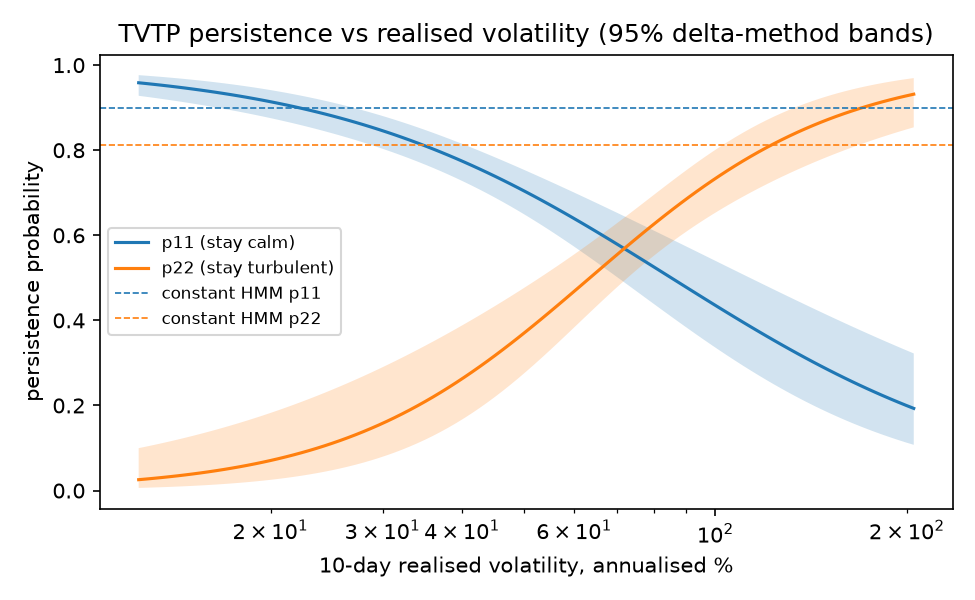
\includegraphics[width=0.62\textwidth]{../results/btc/fig_transition_response.png}
\caption{Estimated persistence probabilities $p_{11}(z)$ (stay calm) and $p_{22}(z)$ (stay turbulent) of the full-sample TVTP model as a function of ten-day realised volatility, with 95\% delta-method bands. Dashed lines: the constant HMM.}\label{fig:response}
\end{figure}

Regime dating around known events is a check on the model, not evidence of foresight. Ten days before the FTX collapse (8 November 2022) the smoothed probability of the turbulent regime was \FTXpre; the filtered probability, causal in the data but computed with full-sample parameters, spiked to 0.8 on \FTXfirst\ on a 4.6\% up-move, fell back below 0.15 the next day, and reached one on 8 November, the day of the 10\% fall, staying above 0.95 through 11 November. The filter reacts on the day, as a daily filter must. Before the 12 March 2020 crash the picture is different: the late-February drawdown had already pushed the filtered probability above 0.9 on 26 February and 8 March, and the smoothed probability ten days before the crash was \COVIDpre. Figure~\ref{fig:dating} shows the full-sample dating and a filtered zoom on 2022; the visible difference between the models after FTX is the TVTP model's longer stay in the turbulent regime, a direct consequence of $\beta_{2,\mathrm{RV}}>0$.

\begin{figure}[t]\centering
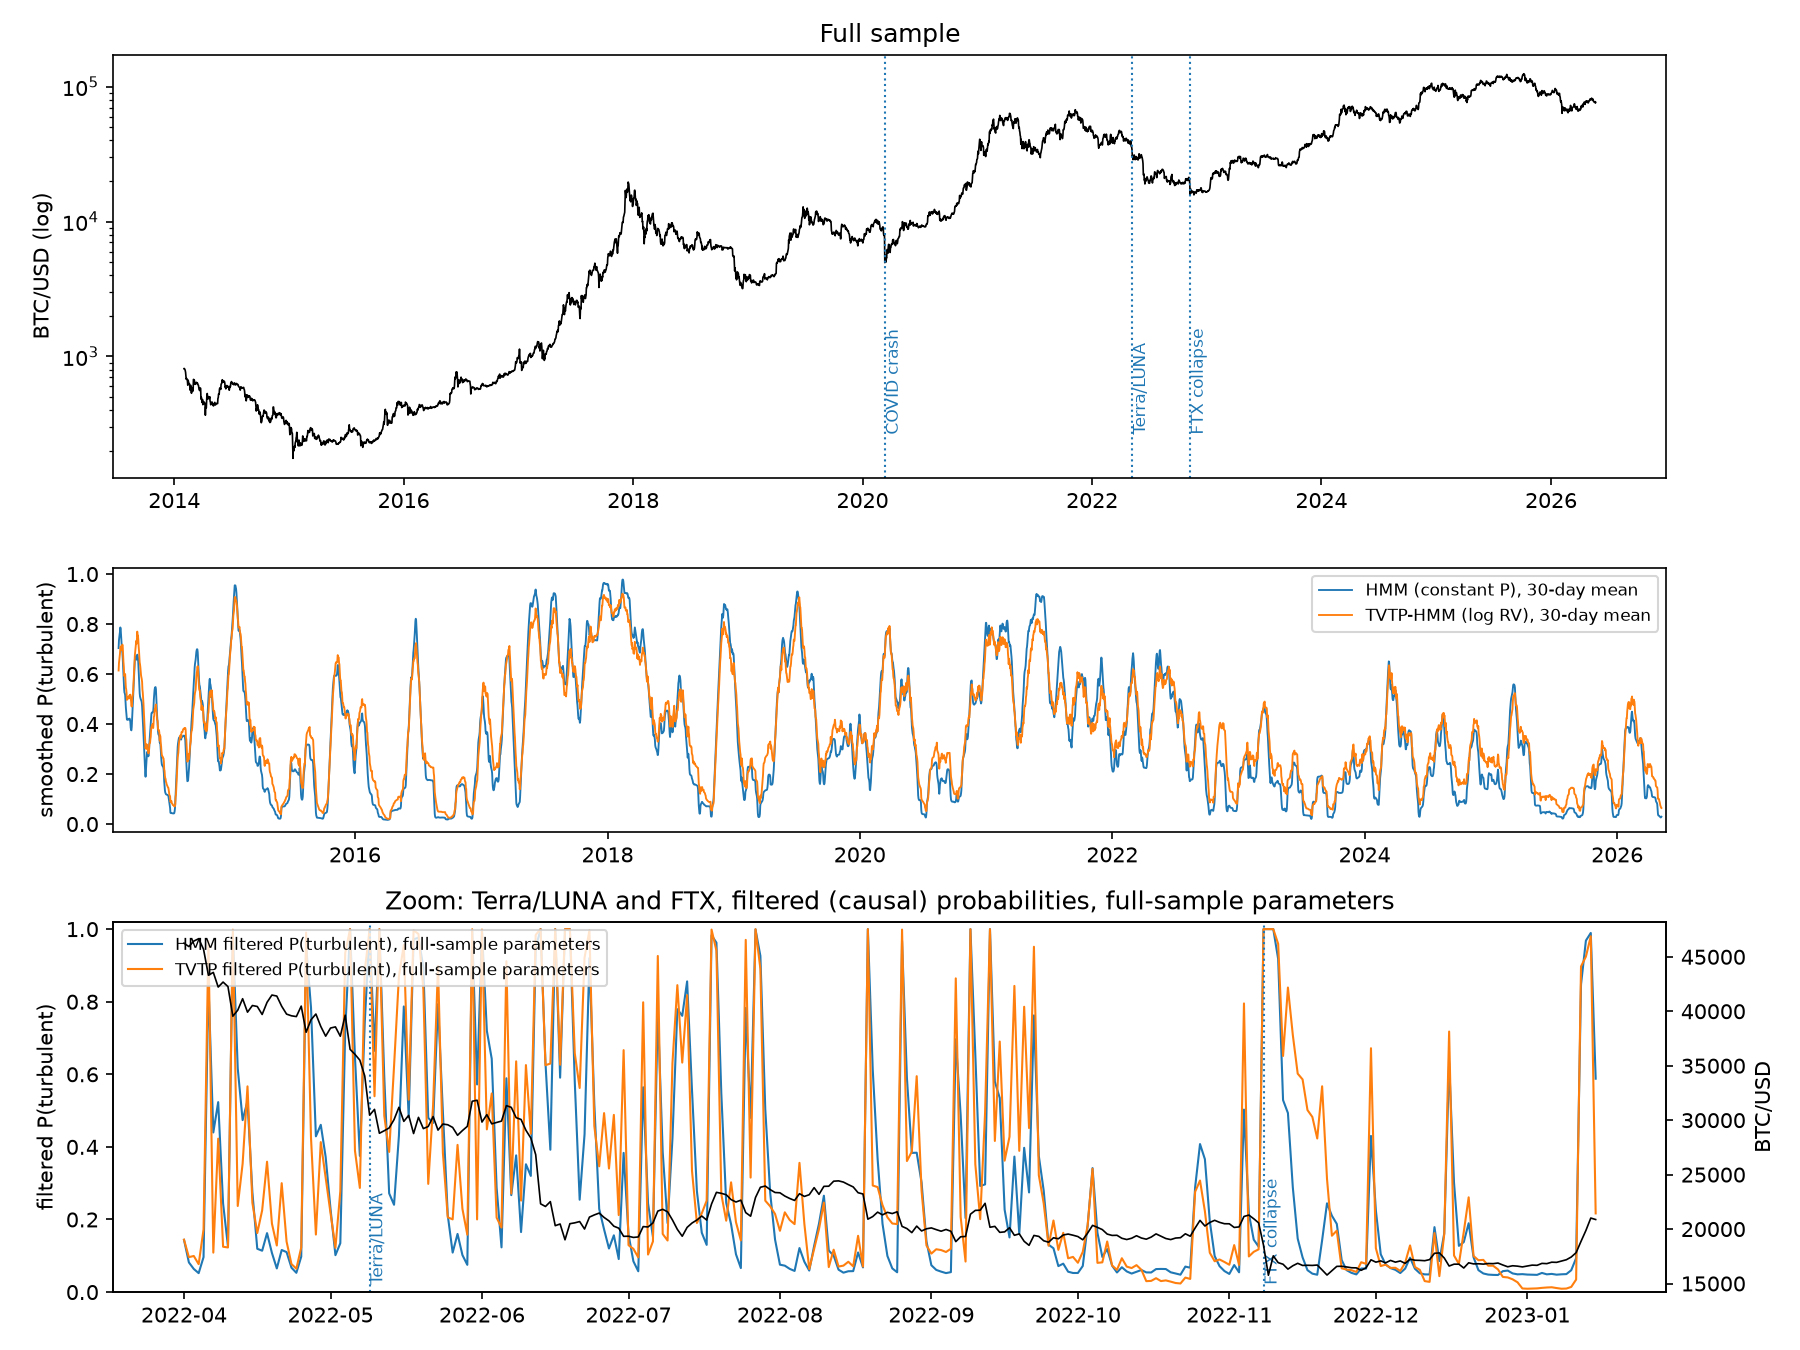
\includegraphics[width=0.95\textwidth]{../results/btc/fig_regime_dating.png}
\caption{Top: BTC/USD (log scale) with the three reference events. Middle: 30-day mean of the smoothed turbulent-regime probability, constant HMM and TVTP model. Bottom: filtered turbulent-regime probabilities around the Terra and FTX events (causal in the data, full-sample parameters).}\label{fig:dating}
\end{figure}

\subsection{Out-of-sample forecasting}
\begin{table}[t]\centering\small
\caption{Out-of-sample one-day-ahead variance and density forecasts, 2018-01-31 to 2026-05-23 (3035 days, 34 refits). Proxy for realised variance: squared daily return. DM statistics test each row against the constant HMM (negative favours the row); HLN small-sample correction, Newey--West bandwidth $\lfloor T^{1/3}\rfloor$. Reference forecasts use no regime model. $^{***}$, $^{**}$, $^{*}$: 1, 5, 10\%.}\label{tab:fc}
\begin{tabular}{lrrrrrr}\toprule Model & QLIKE & MSE ($\times10^{6}$) & Log score & DM QLIKE & DM MSE & DM log score \\ \midrule
Constant HMM & -5.8193 & 22.54 & 2.0996 & -- & -- & -- \\
TVTP, log RV & -5.8816 & 22.28 & 2.1196 & -2.27$^{**}$ & -2.55$^{**}$ & -4.62$^{***}$ \\
TVTP, exchange flow & -5.8258 & 22.53 & 2.0991 & -0.99$^{}$ & -0.13$^{}$ & 0.64$^{}$ \\
TVTP, both & -5.8887 & 22.25 & 2.1196 & -2.24$^{**}$ & -2.34$^{**}$ & -4.60$^{***}$ \\
Rolling RV$_{10}$ (ref.) & -5.5007 & 23.93 & -- & 3.47$^{***}$ & 1.16$^{}$ & -- \\
EWMA(0.94) (ref.) & -5.8250 & 22.54 & -- & -0.13$^{}$ & -0.00$^{}$ & -- \\
\bottomrule\end{tabular}\end{table}

Across the \NWindows\ walk-forward windows the realised-volatility TVTP model rejects the constant HMM at the 5\% level in \WFfracLR\% of windows (median LR \WFmedLR) and has the lower BIC in \WFfracBIC\%; the slopes are stable in sign, ranging from \SlopeOneMin\ to \SlopeOneMax\ for $\beta_{1,\mathrm{RV}}$ and \SlopeTwoMin\ to \SlopeTwoMax\ for $\beta_{2,\mathrm{RV}}$. The exchange-flow model rejects the baseline in \WFfracLRex\% of windows.

Table~\ref{tab:fc} evaluates the one-day-ahead forecasts on the \NOOS\ out-of-sample days. The realised-volatility TVTP model improves on the constant HMM under every loss, and the Diebold--Mariano tests reject equal accuracy: QLIKE $t=\DMqlike$ ($p=\DMqlikeP$), MSE $t=\DMmse$ ($p=\DMmseP$) and predictive log score $t=\DMls$ ($p\DMlsP$). The log-score result is the strongest, as expected: the TVTP model changes the regime-probability forecast, which the density loss measures directly, while the variance forecast is a coarser summary. The exchange-flow model is indistinguishable from the baseline and the combined model adds nothing to realised volatility alone. Two reference forecasts calibrate the magnitudes: the constant HMM is statistically indistinguishable from an EWMA(0.94) variance forecast, whereas the TVTP model beats the ten-day rolling realised variance decisively (QLIKE $t=\DMrvQ$) and is better than EWMA in point but not significantly ($t=\DMewmaQ$, $p=\DMewmaQP$). Allowing the transitions to vary is what lifts the regime model above the naive volatility filters that a practitioner would otherwise use.

\subsection{Trading performance and significance}
\begin{table}[t]\centering\small
\caption{Out-of-sample strategy performance, 2018-01-31 to 2026-05-23, proportional cost 10~bps per unit turnover, long-only. Panel A: primary rule, eq.~(\ref{eq:rule}), target volatility 20\%, cap 1. Panel B: capped-Kelly rule, eq.~(\ref{eq:kelly}), $\gamma=2$. Sharpe and Sortino annualised (365 days).}\label{tab:strat}
\begin{tabular}{lrrrrrr}\toprule Strategy & Ann. return & Ann. vol & Sharpe & Sortino & Max DD & Turnover/yr \\ \midrule
\multicolumn{7}{l}{\textit{Panel A: proportional rule}} \\
\quad Buy and hold & 45.2\% & 63.9\% & 0.71 & 0.95 & -77\% & 0.1 \\
\quad Volatility target, no regime & 10.7\% & 18.2\% & 0.59 & 0.79 & -32\% & 10.2 \\
\quad Constant HMM & 4.6\% & 11.7\% & 0.39 & 0.49 & -25\% & 16.5 \\
\quad TVTP, log RV & 7.0\% & 11.3\% & 0.61 & 0.81 & -25\% & 9.2 \\
\quad TVTP, exchange flow & 4.6\% & 11.8\% & 0.39 & 0.50 & -27\% & 18.1 \\
\quad TVTP, both & 6.8\% & 11.4\% & 0.60 & 0.79 & -25\% & 12.3 \\
\multicolumn{7}{l}{\textit{Panel B: capped Kelly}} \\
\quad Constant HMM & 20.3\% & 39.2\% & 0.52 & 0.62 & -59\% & 37.1 \\
\quad TVTP, log RV & 28.4\% & 37.2\% & 0.76 & 1.00 & -55\% & 19.2 \\
\quad TVTP, exchange flow & 19.6\% & 39.0\% & 0.50 & 0.61 & -63\% & 38.9 \\
\quad TVTP, both & 28.2\% & 37.2\% & 0.76 & 1.00 & -57\% & 24.3 \\
\bottomrule\end{tabular}\end{table}

\begin{table}[t]\centering\small
\caption{Inference on strategy performance. PSR: probability that the true Sharpe exceeds zero. DSR: deflated Sharpe ratio, benchmark $\mathrm{SR}_0$ = expected maximum Sharpe among the $N=54$ configurations tried (both rules, all targets, caps, risk aversions and models). Bootstrap: stationary block bootstrap (2000 draws, mean block 20 days) of the annualised Sharpe difference against the constant-HMM strategy under the same rule.}\label{tab:sig}
\begin{tabular}{llrrrrr}\toprule Rule & Model & Sharpe & PSR & DSR & $\Delta$SR vs HMM [95\% CI] & $p$ \\ \midrule
Proportional & TVTP, log RV & 0.61 & 0.96 & 0.84 & 0.22 [-0.05, 0.49] & 0.107 \\
Proportional & TVTP, exchange flow & 0.39 & 0.87 & 0.64 & -0.00 [-0.08, 0.07] & 0.929 \\
Proportional & TVTP, both & 0.60 & 0.96 & 0.83 & 0.20 [-0.07, 0.47] & 0.131 \\
Proportional & Constant HMM & 0.39 & 0.87 & 0.64 & -- & -- \\
Capped Kelly & TVTP, log RV & 0.76 & 0.99 & 0.92 & 0.25 [0.00, 0.47] & 0.050 \\
Capped Kelly & TVTP, exchange flow & 0.50 & 0.92 & 0.75 & -0.02 [-0.08, 0.04] & 0.571 \\
Capped Kelly & TVTP, both & 0.76 & 0.99 & 0.92 & 0.24 [-0.01, 0.46] & 0.058 \\
\bottomrule\end{tabular}\end{table}

\begin{table}[t]\centering\small
\caption{Annualised Sharpe ratio of the proportional rule as a function of the transaction cost.}\label{tab:cost}
\begin{tabular}{rrrrrr}\toprule Cost (bps) & Buy and hold & Vol target & Constant HMM & TVTP, log RV & Difference \\ \midrule
0 & 0.71 & 0.64 & 0.53 & 0.70 & +0.16 \\
10 & 0.71 & 0.59 & 0.39 & 0.61 & +0.22 \\
25 & 0.71 & 0.50 & 0.18 & 0.49 & +0.31 \\
50 & 0.71 & 0.36 & -0.17 & 0.29 & +0.46 \\
\bottomrule\end{tabular}\end{table}

Table~\ref{tab:strat} reports strategy performance. Under the proportional rule (\ref{eq:rule}) the TVTP strategy earns a Sharpe ratio of \SRtvtp\ against \SRhmm\ for the constant HMM, with turnover of \TOtvtp\ versus \TOhmm\ times per year: because the turbulent regime is more persistent when volatility is high, the TVTP regime probabilities flip less often, and the strategy trades about half as much. Buy-and-hold reaches \SRbh\ over a sample dominated by two bull runs, with a \MDDbh\% drawdown, while the regime rules cap drawdown near \MDDtvtp\% at \VolTvtp\% realised volatility. Regime conditioning through $\xi_{t|t-1}(1)$ double-counts turbulence already priced into $h_{t|t-1}$, which is why the volatility-target benchmark without regime conditioning outperforms the constant-HMM rule; the TVTP model recovers that gap. Under the capped-Kelly rule (\ref{eq:kelly}), which conditions on regimes only through the mixture moments, the TVTP strategy reaches \SRtvtpK\ against \SRhmmK\ for the constant HMM and \SRbh\ for buy-and-hold, with a \MDDtvtpK\% drawdown at \VolTvtpK\% volatility and \WealthTvtpK$\times$ terminal wealth against \WealthBH$\times$.

Table~\ref{tab:sig} contains the inference. The TVTP strategies have probabilistic Sharpe ratios of \PSR\ (proportional) and \PSRK\ (Kelly) against zero, and deflated Sharpe ratios of \DSR\ and \DSRK\ once the expected maximum Sharpe of $\SRzero$ among $N=\NTrials$ trials is used as the benchmark. The quantity the research question asks about is the difference to the constant HMM under the same rule: \BootDiff\ with bootstrap 95\% interval [\BootLo, \BootHi] ($p=\BootP$) for the proportional rule and \BootDiffK\ with [\BootLoK, \BootHiK] ($p=\BootPK$) for the Kelly rule. The improvement is economically meaningful and borderline significant at the 5\% level. Table~\ref{tab:cost} shows that it is not an artefact of low costs: the Sharpe gap between the TVTP and constant-HMM strategies widens from \GapZero\ at zero cost to \GapFifty\ at 50~bps, because the constant HMM pays for its extra turnover.

\subsection{Robustness: three regimes and Student-$t$ emissions}\label{sec:robust}
\paragraph{Three regimes.} \KthreeText

Two things change and one does not. The density-forecast improvement is robust: the log-score test rejects at any conventional level with either regime count, consistent with the mechanism in Section~\ref{sec:method}, where time variation changes the regime-probability forecast rather than the regime moments. The variance-forecast improvement weakens (MSE remains significant, QLIKE does not), and the trading improvement disappears: the three-regime constant HMM is a much better trading model than its two-regime counterpart (Sharpe \KthreeSRhmm\ against \SRhmm\ under the proportional rule, \KthreeSRhmmK\ against \SRhmmK\ under Kelly), which closes most of the gap that time variation closes at $K=2$, and adding time variation to it changes the Sharpe ratio by an amount whose bootstrap interval is centred near zero. The intermediate regime absorbs most of what the covariate contributes to the two-regime model, namely the ability to stay out of the calm state while volatility is elevated.

\paragraph{Student-$t$ emissions.} \StudentTText

The two checks point the same way. Time-varying persistence driven by realised volatility is a genuine feature of the data: its full-sample likelihood-ratio statistic is far beyond any critical value under either emission, and its slopes keep their sign and grow when the tails are modelled. But its out-of-sample value depends on what the baseline lacks. Against a two-regime Gaussian HMM, which cannot represent elevated-but-not-extreme volatility except by switching, the covariate supplies exactly that, and forecasts and trading improve. A third regime or a heavy-tailed emission supplies it too, and better: the $t$-HMM's predictive log score exceeds the Gaussian TVTP model's, and once either is in place the covariate has little left to add within a four-year estimation window, where its slopes are poorly identified. This is the identification difficulty documented by \citet{modee2026} appearing in the wild. The trading conclusion of Section~\ref{sec:results} is therefore specific to the two-regime Gaussian specification and is stated as such.

\section{Discussion and limitations}\label{sec:discussion}
The evidence separates into three layers. Statistically, time variation in the transition probabilities driven by realised volatility is a large and stable effect in the full sample: its sign never flips and it survives both a third regime and heavy-tailed emissions. Predictively, against the two-regime Gaussian baseline the improvement is significant on every loss and is what lifts the regime model above naive volatility filters, but against a three-regime or Student-$t$ baseline it shrinks to the density loss or disappears. Economically, with two Gaussian regimes the improvement over the constant HMM is of the order of a quarter of a Sharpe unit with half the turnover, borderline significant under both rules (bootstrap $p=\BootPK$ and $p=\BootP$, the first sensitive to the bootstrap seed and block length); with three regimes or $t$ emissions it vanishes. Nothing stronger is supported: no long-only volatility-targeted rule beats buy-and-hold on Sharpe over a sample of this kind, though all of them cut the drawdown substantially, and the on-chain exchange-flow covariate carries no out-of-sample information.

The pattern has a simple reading. A two-regime Gaussian HMM with fixed transitions is a coarse volatility filter, indistinguishable from EWMA out of sample; it lacks a way to represent elevated-but-not-extreme volatility other than by switching. Time-varying persistence supplies that, and so do an intermediate regime or heavy tails, and the latter do it with fewer parameters that are better identified in a four-year window. The point ranking of the three fixes by out-of-sample log score, $t$ emission first, then time variation, then a third regime, is suggestive rather than established: the $t$-HMM's margin over the Gaussian TVTP model has a Diebold--Mariano statistic of $t=\XDMtls$ ($p=\XDMtlsP$), and the Gaussian TVTP and three-regime models are indistinguishable ($t=\XDMkls$, $p=\XDMklsP$). Read that way, tail thickness within a regime matters at least as much for Bitcoin as the timing of switches between regimes. This is consistent with \citet{modee2026}, who find one-step forecasts robust to the transition specification and the transition coefficients hard to identify.

Limitations follow from the design choices. Prices are daily reference rates rather than exchange OHLC, so range-based realised-volatility estimators and intraday variance proxies were unavailable and the squared return, a noisy proxy, is used; QLIKE mitigates but does not remove the resulting loss of power. The Student-$t$ variance forecast $\sigma_j^2\nu_j/(\nu_j-2)$ is fragile when $\hat\nu_j$ is near two, as it is in the calm regime, which penalises the $t$ models on the variance losses and in the volatility-scaled rule; a robust scale would be the fairer input to the allocation rule. The transaction-cost model is proportional and ignores market impact. Two Gaussian regimes are the main specification although BIC favours three regimes and, more strongly, $t$ emissions; Section~\ref{sec:robust} shows that the choice matters for everything beyond the full-sample fit. A three-regime $t$-emission TVTP model with regime-specific allocation weights is the natural continuation, as is a covariate that is not itself a function of past returns, since realised volatility competes most directly with what the emission distribution already captures. The three-regime run used EM without the quasi-Newton polish and three restarts per window, so its point estimates carry more Monte Carlo noise than the two-regime runs. The deflated Sharpe ratio counts \NTrials\ trials, which covers the configurations reported and their siblings but not the design decisions taken before any backtest was run; pooling the \NTrialsAll\ configurations backtested across the main, three-regime and Student-$t$ runs leaves the deflated ratios at \DSRpooled\ and \DSRKpooled, because the pooled trial variance is smaller. The regularity of the likelihood-ratio test presumes that the constant $K$-regime model is identified; with fewer genuine regimes than $K$ the test is oversized. Finally, the study covers one asset over one eight-year out-of-sample period; the qualitative mechanism, stress-dependent regime persistence, should transfer to other assets, but the trading conclusions should not be extrapolated.

\section{Conclusion}\label{sec:conclusion}
Letting the transition probabilities of a Bitcoin volatility HMM depend on lagged realised volatility is a one-line change to the Hamilton filter with a closed-form-adjacent EM step, a regular likelihood-ratio test, and an estimator whose finite-sample behaviour matches theory. On Bitcoin the effect is strong and stable: calm regimes end sooner and turbulent regimes last longer as volatility rises. Against the standard two-regime Gaussian HMM this improves one-day-ahead variance and density forecasts significantly under strict walk-forward validation and translates into a regime-conditioned allocation rule with higher Sharpe ratio and lower turnover, an improvement that is economically meaningful and borderline significant once selection bias and dependence are accounted for. Against richer baselines the gain shrinks: a third regime keeps the density gain and loses the trading gain, and Student-$t$ emissions, the change that improves the model most, leave nothing for time variation to add out of sample. The answer to the research question is therefore split. Time-varying transition probabilities are a real and well-identified feature of Bitcoin's regime dynamics, and the covariate that carries them is realised volatility rather than on-chain flow; but their forecasting and trading value is conditional on a baseline that cannot otherwise represent elevated volatility, and a properly specified emission distribution is the more effective fix. That conclusion could not have been reached from fit statistics alone, which is the case for the evaluation design used here. The companion repository reproduces every number in this document from public data in under an hour.

\setlength{\bibsep}{3pt}
{\small\bibliographystyle{abbrvnat}
\bibliography{refs}}
\end{document}
